\chapter{Architecture}
\begin{figure}[htbp]
    \centering
    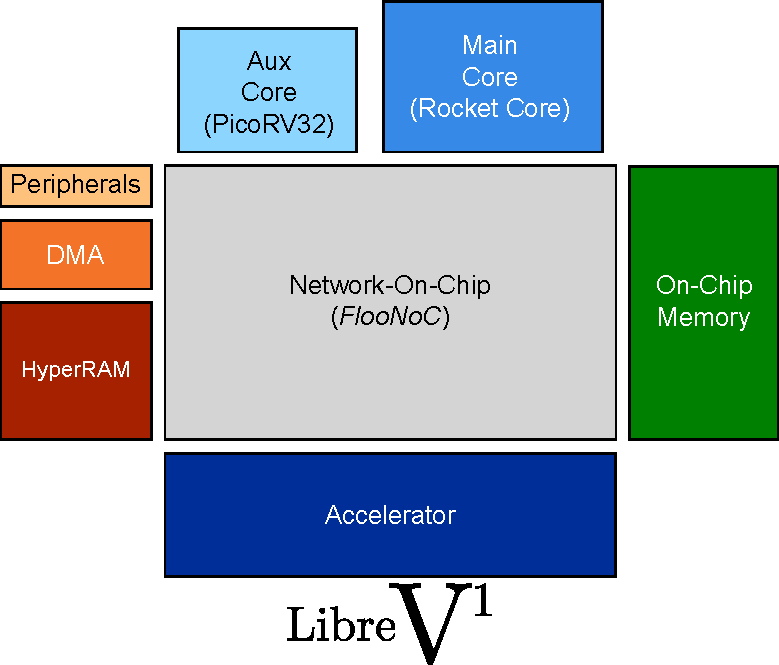
\includegraphics[width=0.65\textwidth]{figures/libre_concept.pdf}
    \caption{Libre-V system-on-chip concept.}
    \label{fig:soc-concept}
\end{figure}

\section{Overview}
Libre-V is a configurable system-on-chip platform intended to be used as host-CPU for testing ASICs, especially accelerators. Being composed of all open-source components, it is completely open source and licensed under the Apache-2.0 license\footnote{Individual components may be protected by their own licensing. Refer the \href{https://code.stanford.edu/tambe-lab/base-soc-v2/-/blob/main/README.md}{repository} for more details.}. The platform uses a 32-bit auxilary core coupled with a 64-bit main core. The auxilary core implements RV32IMC instruction set, whereas the main core implements RV64GC instruction set.  

\begin{docwarning}
    This is document does not discuss the implementation of either the RISC-V ISA nor any of the individual SoC components. For that, we direct the reader to the documentation available at \href{https://riscv.org/specifications/ratified/}{respective source(s)}.  
\end{docwarning}

\section{System}

\begin{figure}[htbp]
  \centering
  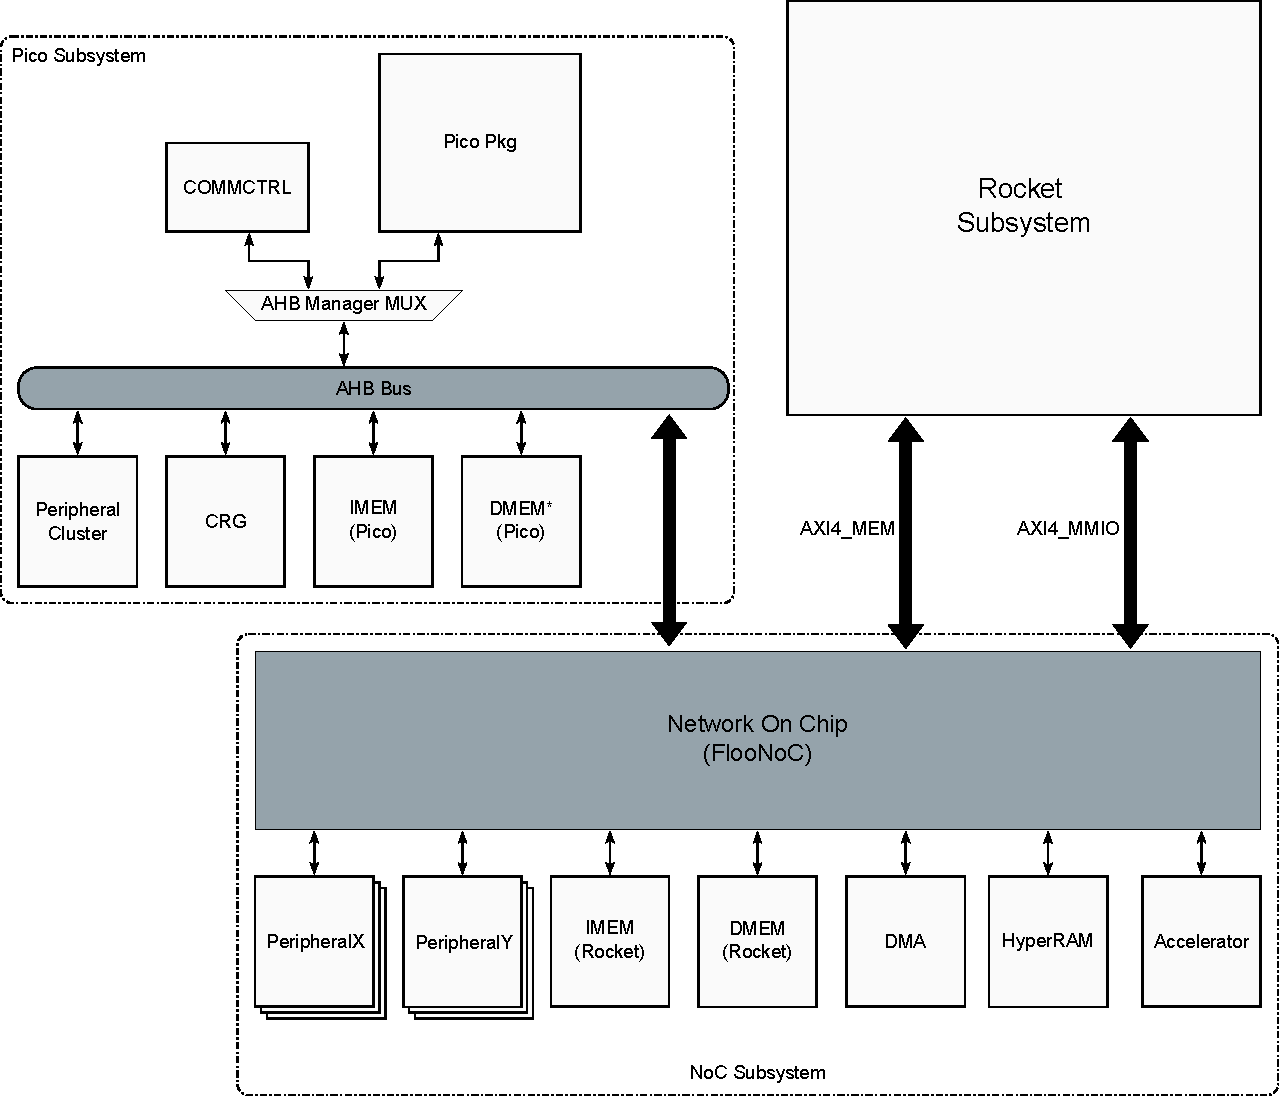
\includegraphics[width=0.95\textwidth]{figures/libre_top_blk.pdf}
  \caption{Libre-V platform block view.}
  \label{fig:top-blk}
\end{figure}

Libre-V platform has 32-bit address space shared by memory-mapped I/O devices. It is composed of three subsystems: 

\begin{enumerate}
    \item Pico Subsystem
    \item Rocket Subsystem 
    \item Network on Chip (NoC) Subsystem
\end{enumerate}

See Figure~\ref{fig:top-blk} for a block-view of the platform. Note that the figure only shows two peripheral groups in the NoC subsystem. However, this is only meant for illustrations. It is possible to configure an Libre-V instance with more than 2 peripherals.

This part of the manual provides a software view of each  component of the Libre-V:  
\begin{itemize}
    \item \hyperref[ch:sw-pico-sys]{Pico Subsystem}
    \item \hyperref[ch:sw-rocket-sys]{Rocket Subsystem}
    \item \hyperref[ch:sw-uart]{UART}
    \item \hyperref[ch:sw-timer]{Timer}
    \item \hyperref[ch:compiling-firmware]{Libre Firmware and Device Drivers}
    \item \hyperref[ch:libre-boot]{Libre Booting Process}     
\end{itemize}
% TODO: Fix all the forward links and add the new entries. 

\newpage
